\documentclass[12pt]{article}
\usepackage{amsmath}
\usepackage{amssymb}
\usepackage{cancel}
\usepackage{graphicx}
% \usepackage{physics}
\usepackage{siunitx}
\usepackage{wrapfig}

% \AtBeginDocument{\RenewCommandCopy\qty\SI}

\newcommand{\E}[1]{\times 10^{#1}}

\title{
    Chapter 17 End-of-Chapter Problems
    \\ \small
    Halliday \& Resnick, 10th Edition
}

\author{Donald Aingworth IV}

\date{\small Hit me where it Matters}

\begin{document}
    \DeclareSIUnit{\atm}{atm}
    \DeclareSIUnit{\cal}{\ cal}
    \DeclareSIUnit{\Cal}{\ Cal}
    \DeclareSIUnit{\calorie}{\ cal}
    \DeclareSIUnit{\Calorie}{\ Cal}
    \DeclareSIUnit{\celsiusdegree}{C^\circ}
    \DeclareSIUnit{\fahrenheit}{^\circ F}
    \DeclareSIUnit{\fahrenheitdegree}{F^\circ}
    \DeclareSIUnit{\torr}{\ torr}

    \maketitle

    \begin{center}
        \textit{Where needed in the problems, use}\\
        speed of sound in air = 343 m/s\\
        \textit{and}\\
        density of air = 1.21 \unit{\kilo\gram/\meter^3}\\
        \textit{unless otherwise specified.}
    \end{center}

    \pagebreak
    \section{Problem 1}
        Two spectators at a soccer game see, and a moment later hear, the ball being kicked on the playing field. 
        The time delay for spectator A is 0.23 s, and for spectator B it is 0.12 s. 
        Sight lines from the two spectators to the player kicking the ball meet at an angle of 90\unit{\degree}. 
        How far are (a) spectator A and (b) spectator B from the player?
        (c) How far are the spectators from each other?

        \subsection{Solution (a)}
            This is a simple question to answer.
            The distance traveled to A would be equal to the speed of sound times the time taken to travel the distance.
            \begin{align}
                x   &=  vt
                    =   (343\,\unit{\meter/\second})(0.23\,\unit{\second})
                    =   \boxed{78.89\,\unit{\meter}}
            \end{align}

        \subsection{Solution (b)}
            The is calculatable the same way.
            \begin{equation}
                y   =   vt
                    =   (343\,\unit{\meter/\second})(0.12\,\unit{\second})
                    =   \boxed{41.16\,\unit{\meter}}
            \end{equation}

        \subsection{Solution (c)}
            The 90 degree angle of their sight lines makes the triange of the two spectators and the ball a right triangle, so we can use the Pythagorean theorem to find the distance between the spectators.
            \begin{equation}
                h   =   \sqrt{x^2 + y^2}
                    =   \sqrt{(78.89\,\unit{\meter})^2 + (41.16\,\unit{\meter})^2}
                    =   \boxed{88.98\,\unit{\meter}}
            \end{equation}

    \pagebreak
    \section{Problem 3}
        When the door of the Chapel of the Mausoleum in Hamilton, Scotland, is slammed shut, the last echo heard by someone standing just inside the door reportedly comes 15 s later. 
        (a) If that echo were due to a single reflection off a wall opposite the door, how far from the door is the wall? 
        (b) If, instead, the wall is 25.7 m away, how many reflections (back and forth) occur?

        \subsection{Solution (a)}
            Use the speed and the time taken to calculate the distance covered.
            \begin{align}
                \Delta s    &=  vt
                    =   (343\,\unit{\meter/\second}) (15\,\unit{\second})
                    =   5145\,\unit{\meter}
            \end{align}

            This is twice the length of the church, so if we divide this by two, we will get the length of the church.
            \begin{equation}
                L   =   \frac{\Delta s}{2}
                    =   \frac{5145\,\unit{\meter}}{2}
                    =   \boxed{2572.5\,\unit{\meter}}
            \end{equation}

        \subsection{Solution (b)}
            We can divide the total distance covered by the length of the church to fnd the number of reflections.
            \begin{align}
                n   &=  \frac{5145\,\unit{\meter}}{25.7\,\unit{\meter}}
                    =   200.19\\
                \lfloor n \rfloor   &=  \boxed{200}
            \end{align}

    \pagebreak
    \section{Problem 5}
        Earthquakes generate sound waves inside Earth.
        Unlike a gas, Earth can experience both transverse (S) and longitudinal (P) sound waves. 
        Typically, the speed of S waves is about 4.5 km/s, and that of P waves 8.0 km/s. 
        A seismograph records P and S waves from an earthquake. 
        The first P waves arrive 3.0 min before the first S waves. 
        If the waves travel in a straight line, how far away did the earthquake occur?

        \subsection{Solution}
            3.0 minutes is equivalent to 180 seconds.
            If the time it takes the longitudinal wave to reach the scale is $t$, the time it takes the transverse wave would be $t + 180\,\unit{\second}$. 
            We can use this in an equation for distance from velocity.
            \begin{gather}
                \Delta x    =   vt\\
                x   =   (8.0\,\unit{\kilo\meter/\second})t\\
                x   =   (4.5\,\unit{\kilo\meter/\second})(t + 180\,\unit{\second})
            \end{gather}

            Use the transistive property and solve for the time.
            \begin{gather}
                (8.0\,\unit{\kilo\meter/\second})t  =   (4.5\,\unit{\kilo\meter/\second})(t + 180\,\unit{\second})\\
                (3.5\,\unit{\kilo\meter/\second})t  =   810\,\unit{\kilo\meter}
                    =   \frac{810}{3.5}\,\unit{\second}
            \end{gather}
            
            Substitute this into the first equation for the distance covered.
            \begin{align}
                x   &=  (8.0\,\unit{\kilo\meter/\second})(\frac{810}{3.5}\,\unit{\second})
                    =   \boxed{1851\,\unit{\kilo\meter}}
            \end{align}

    \pagebreak
    \section{Problem 7}
        A stone is dropped into a well. 
        The splash is heard 3.00 s later. 
        What is the depth of the well?

        \subsection{Solution}
            The time taken of 3.00 s is the time taken for the stone to drop plus the time taken for the sound to return up the well.
            We can create formulas for each of these, using a gravitational constant of $9.81\,\unit{\meter/\second^2}$.
            \begin{gather}
                h   =   \frac{1}{2}gt_1^2
                    =   \frac{(9.81\,\unit{\meter/\second^2})}{2} t_1^2\\
                h   =   vt_2
                    =   (343\,\unit{\meter/\second})t_2\\
                t_1 + t_2   =   3.00\,\unit{\second} \to
                t_2 =   3.00\,\unit{\second} - t_1
            \end{gather}

            We can substitute our value of $t_2$ into the equation for the distance traveled by the sound and solve that for $t_1$.
            \begin{gather}
                h   =   (343\,\unit{\meter/\second}) (3.00\,\unit{\second} - t_1)\\
                3.00\,\unit{\second} - t_1  =   \frac{h}{343\,\unit{\meter/\second}}\\
                t_1 =   3.00\,\unit{\second} - \frac{h}{343\,\unit{\meter/\second}}
            \end{gather}

            This in turn can be substituted into our other equation for the depth of the well.
            \begin{gather}
                h   =   \frac{(9.81\,\unit{\meter/\second^2})}{2} t_1^2
                    =   \frac{(9.81\,\unit{\meter/\second^2})}{2} \left( 3.00\,\unit{\second} - \frac{h}{343\,\unit{\meter/\second}} \right)^2\\
                2 (343\,\unit{\meter/\second})^2 h  =   9.81\,\unit{\meter/\second^2} \left( (1029\,\unit{\meter})^2 - (2058\,\unit{\meter})h + h^2 \right)
            \end{gather}

            This gives us a polynomial.
            Solving that polynomial gives us a value of \boxed{h = 40.72\,\unit{\meter}}.

    \pagebreak
    \section{Problem 11}
        Diagnostic ultrasound of frequency 4.50 MHz is used to examine tumors in soft tissue. 
        (a) What is the wavelength in air of such a sound wave? 
        (b) If the speed of sound in tissue is 1500 m/s, what is the wavelength of this wave in tissue?

        \subsection{Solution (a)}
            We have an equation for frequency and wavelength and an accepted speed of sound in air.
            \begin{gather}
                v   =   \lambda f\\
                v   =   343\,\unit{\meter/\second}
            \end{gather}

            We can use these to get the wavelength.
            \begin{align}
                \lambda &=  \frac{v}{f}
                    =   \frac{343\,\unit{\meter/\second}}{4,50\E{6}\,\unit{\hertz}}
                    =   \boxed{7,62\E{-5}\,\unit{\meter}}
            \end{align}

        \subsection{Solution (b)}
            Let's do the same thing.
            \begin{gather}
                v   =   \lambda f\\
                v   =   1500\,\unit{\meter/\second}
            \end{gather}

            We can use these to get the wavelength.
            \begin{align}
                \lambda &=  \frac{v}{f}
                    =   \frac{1500\,\unit{\meter/\second}}{4,50\E{6}\,\unit{\hertz}}
                    =   \boxed{3,3\E{-4}\unit{\meter}}
            \end{align}

    \pagebreak
    \section{Problem 15}
        \begin{wrapfigure}{r}{0.33\textwidth}
            % \vspace{-30pt}
            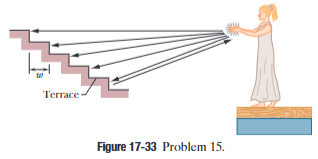
\includegraphics[width=0.33\textwidth]{17-33.png} 
            % \label{fig:wrapfig}
        \end{wrapfigure}
        A handclap on stage in an amphitheater sends out sound waves that scatter from terraces of width $w = 0.75$ m (Fig. 17-33). 
        The sound returns to the stage as a periodic series of pulses, one from each terrace; the parade of pulses sounds like a played note. 
        (a) Assuming that all the rays in Fig. 17-33 are horizontal, find the frequency at which the pulses return (that is, the frequency of the perceived note). 
        (b) If the width $w$ of the terraces were smaller, would the frequency be higher or lower?

        \subsection{Solution (a)}
            With each step, the sound would have to travel an additional distance of $2w$.
            If we divide the speed of all these sounds by the extra distance to travel, we would get the frequency of the return of the pulse rays.
            \begin{equation}
                f   =   \frac{v}{\Delta x}
                    =   \frac{343\,\unit{\meter/\second}}{2(0.75\,\unit{\meter})}
                    =   \boxed{228.67\,\unit{\hertz}}
            \end{equation}
        
        \subsection{Solution (b)}
            The frequency would be higher.

    \pagebreak
    \section{Problem 17}

        \subsection{Solution}

    \pagebreak
    \section{Problem 19}

        \subsection{Solution}

    \pagebreak
    \section{Problem 20}

        \subsection{Solution}

    \pagebreak
    \section{Problem 25}

        \subsection{Solution}

    \pagebreak
    \section{Problem 27}

        \subsection{Solution}

    \pagebreak
    \section{Problem 29}

        \subsection{Solution}

    \pagebreak
    \section{Problem 35}

        \subsection{Solution}

    \pagebreak
    \section{Problem 39}

        \subsection{Solution}

    \pagebreak
    \section{Problem 41}

        \subsection{Solution}

    \pagebreak
    \section{Problem 47}

        \subsection{Solution}

    \pagebreak
    \section{Problem 49}

        \subsection{Solution}

    \pagebreak
    \section{Problem 51}

        \subsection{Solution}

    \pagebreak
    \section{Problem 53}

        \subsection{Solution}

    \pagebreak
    \section{Problem 55}

        \subsection{Solution}

    \pagebreak
    \section{Problem 57}

        \subsection{Solution}

    \pagebreak
    \section{Problem 61}

        \subsection{Solution}

    \pagebreak
    \section{Problem 63}

        \subsection{Solution}

    \pagebreak
    \section{Problem 71}

        \subsection{Solution}

    \pagebreak
    \section{Problem 81}

        \subsection{Solution}

    \pagebreak
    \section{Problem 87}

        \subsection{Solution}

    \pagebreak
    \section{Problem 99}

        \subsection{Solution}

    \pagebreak
    \section{Problem 107}

        \subsection{Solution}

    \pagebreak

    \tableofcontents
\end{document}